\appendix

\section{Annex A : tracking outside of the bandwidth}
\label{annex:tracking}

If the requirements were to track a signal at a frequency higher than the bandwidth of the closed loop, two things could 
have been done. Either we increase the bandwidth or we add a specific part to the controller for it to be effective 
around the desired frequency.

\subsection{Lead compensator}

\begin{align}
    H_{\text{lead}}(s) = \frac{s - z_1}{s - p_1} && z_1 < p_1
\end{align}

A widely used type of regulator is the lead compensator. Its principle is easy to understand thanks to the asymptotic
plot of Bode curves. As the zero comes before the pole, the gain plot will be increasing at this point and the pole is 
just there to ensure causality. The zero must be placed where the amplitude of the transfer function must be increased. 
On the other hand, the pole simply has to be placed far enough to not decrease it where it needs to be high. Here is the 
Bode plot for the closed loop with the zero placed in $600 \text{rad}/s$ (where the magnitude started decreasing) 
and the pole in $1000 \text{rad}/s$:

\begin{figure}[H]
    \centering
    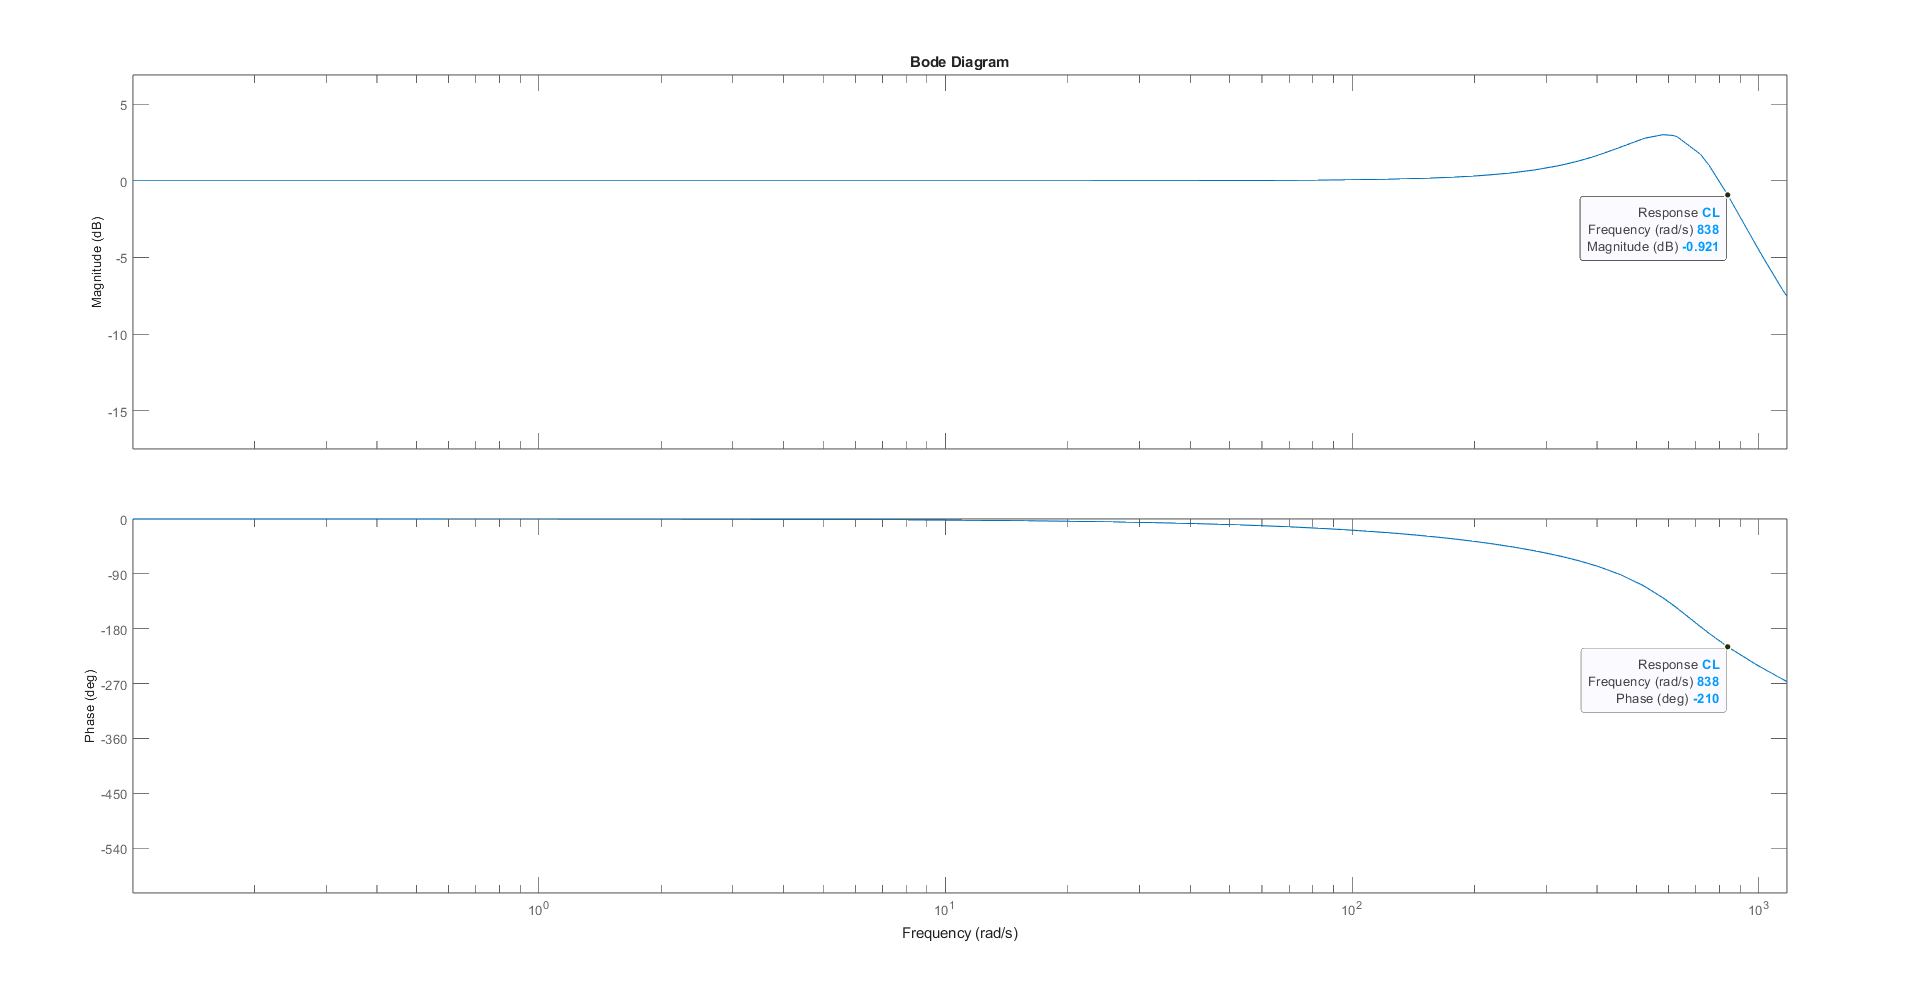
\includegraphics[height=\textheight/3]{Pictures/annex_lead_comp.png}
    \caption{Bode diagram of the closed loop system with a lead compensator $H_{\text{lead}}(s) = \frac{s-600}{s-1000}$}
\end{figure}

This way, the bandwidth has been increased to more than $850 \text{rad}/s$, which is not a significant improve but it
still allows the tracking of faster references.

\subsection{Specific frequency tracker}

\begin{equation}
    H_{\text{spec}}(s) = \frac{1}{s^2 + \omega_{\text{spec}}^2}
\end{equation}

From a theoretical point of view, this regulator is supposed to track perfectly a sine (or cosine) at the pulsation
$\omega_{\text{spec}}$ as it has the same denominator as the reference. However, this transfer function has pure 
imaginary poles. This means that the closed loop system is unstable, despite it having the desired behaviour based on
the Bode plot (magnitude close to $0 dB$ in $\omega_{\text{spec}}$):

\begin{figure}[H]
    \centering
    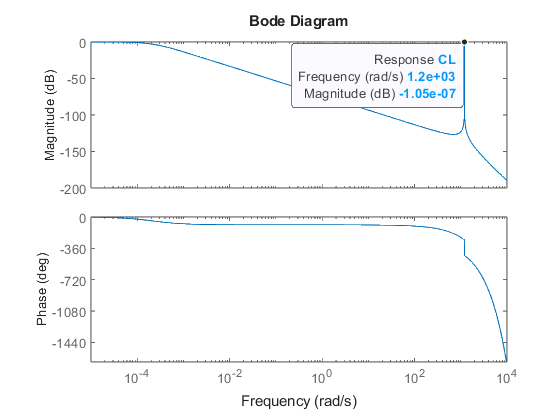
\includegraphics[height=\textheight/3]{Pictures/annex_spec_im.png}
    \caption{Bode diagram of the closed loop system with a specific frequency tracker $H_{\text{spec}}(s) = \frac{1}{s^2
    +1200^2}$}
\end{figure}

It is however really interesting to slightly move these poles away from the imaginary axis and by considering the 
following controller:

\begin{align}
    C(s) &= C_{PI}(s) \times H_{\text{spec}}(s)\\
    &= k_p\times\frac{\tau s + 1}{\tau s(s^2+s+(1200)^2)}
\end{align}

By then following the same methodology as in section \ref{section:freq_analysis}, $k_p = 24\times 10^6$ allows a gain 
of $6 dB$ and the closed loop bandwidth reaches $1300 \text{rad}/s$ as it can be seen on figure 
\ref{fig:spec_ref_tracker}. As this is only an annex, we will stop the analysis here even if this would certainly be 
problematic due to saturation phenomenons\footnote{A simulink simulation would probably prove it}. 

\begin{figure}[H]
    \centering
    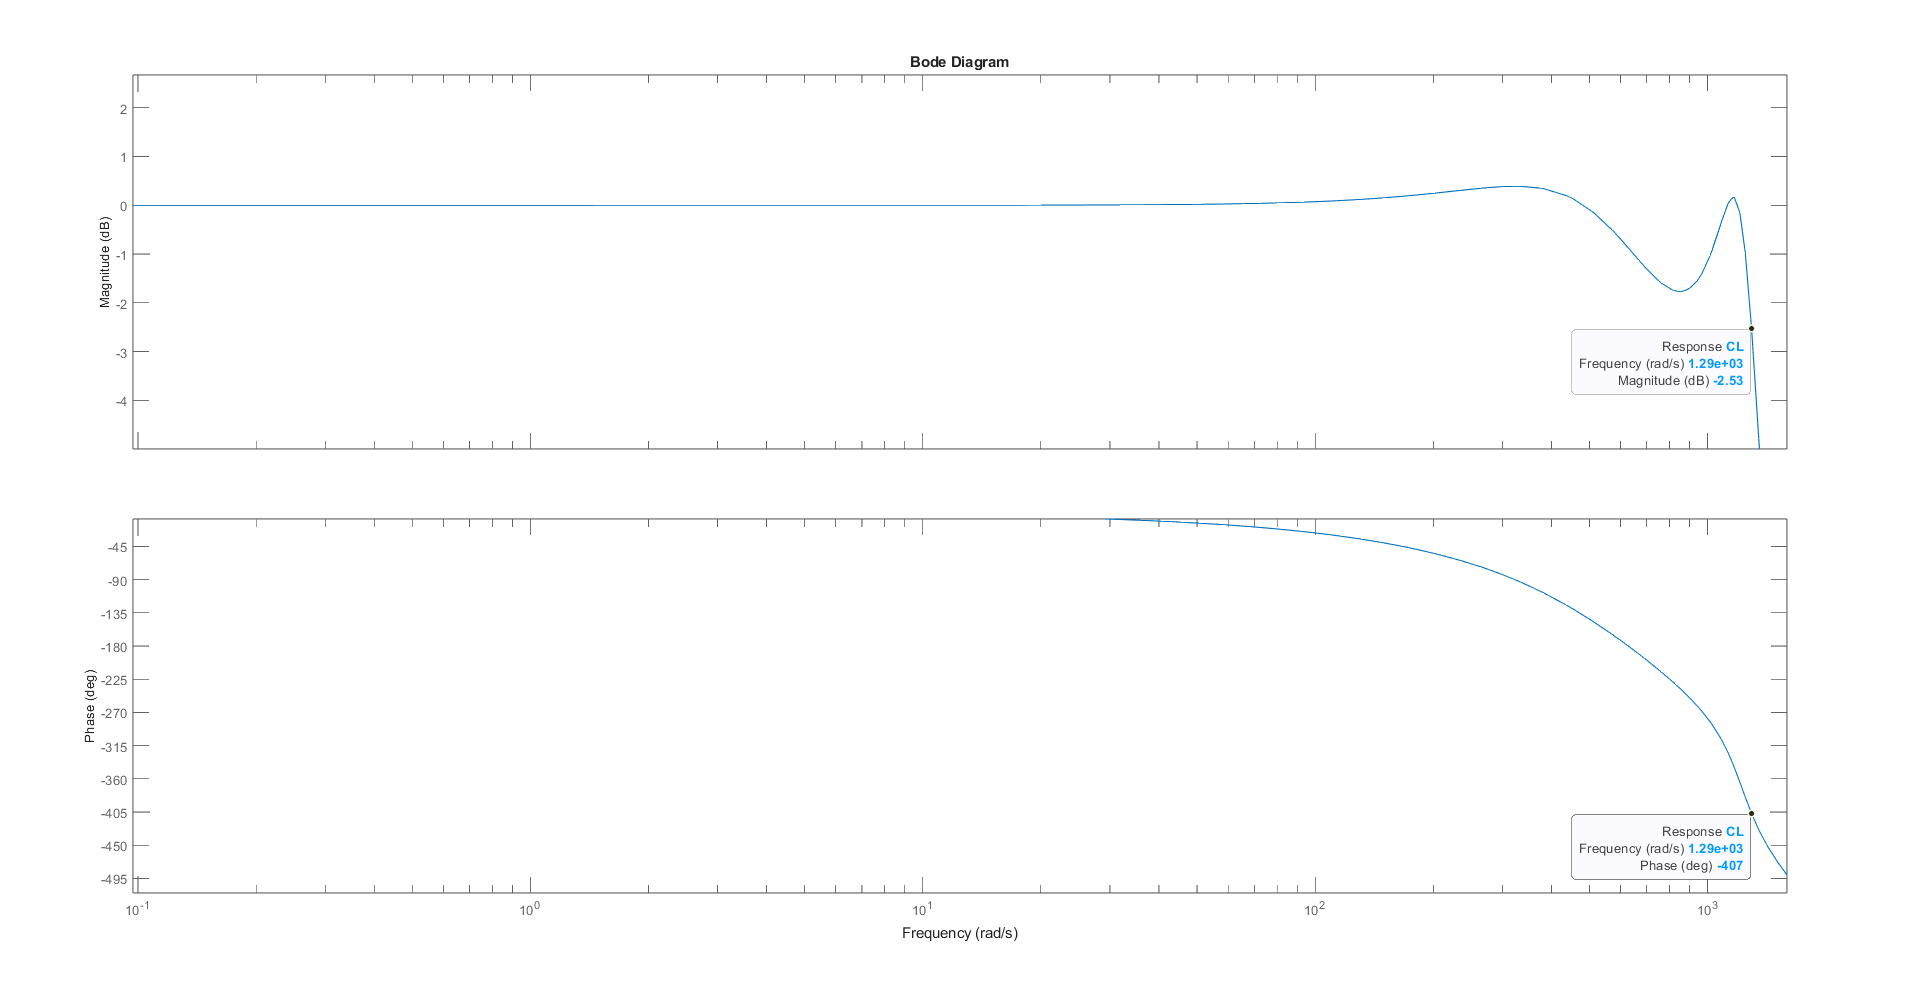
\includegraphics[height=\textheight/3]{Pictures/annex_spec_cmplx.png}
    \caption{Bode diagram of the closed loop system with a specific frequency tracker $H_{\text{spec}}(s) = \frac{1}{s^2
    +s+1200^2}$}
    \label{fig:spec_ref_tracker}
\end{figure}


